\section{Use case validation}\label{sec:experiments}

In this section, we demonstrate the utility of \ac{CLEAVE} by walking readers through an example use case.
With this, we aim to showcase the ability of our framework to provide accurate and repeatable measurements of the performance of \acp{NCS} deployed on edge computing infrastructure.

We present the following use case scenario.
A simple \ac{NCS} consisting of an \emph{inverted pendulum} plant controlled by a \emph{proportional-differential} controller is to be deployed on an Edge server.
The connection between plant and server is over a WiFi (IEEE 802.11n) link.
Moreover, there are a number of video-streaming applications running concurrently on the Edge setup.

We believe this to be an interesting and representative use-case scenario for a number of reasons.
Firstly, the inverted pendulum is broadly used as a benchmark in control-system literature, see for instance\ \cite{Baumann2018LowPower} and\ \cite{Natale2004InvPendEthernet}.
A key reason for this is that such a relatively simplistic system allows for straightforward reparametrization to obtain varied system dynamics, which in turn makes a broader range of experiments possible.
Secondly, similar, albeit non-Edge-enabled, setups have been a reality in industry for almost two decades, as evidenced by\ \cite{Gupta2010NCSOverview}.
Thirdly, although real deployments would most assuredly employ mobile technologies due to the added benefits of mobility and range, the \acp{RTT} offered by these technologies are higher, or at best equal, those offered by WiFi.
4G, for instance, has average \acp{RTT} of around a few hundred milliseconds, which is orders of magnitude greater than the values measured in our scenario, and current 5G deployments offer \ac{RTT} values barely matching the sub-\SI{10}{\milli\second} values we obtain for WiFi.
Thus, we argue that using WiFi allows for more experimental freedom, as the system can be tweaked to obtain worse \acp{RTT} more akin to those of mobile technologies while still having the option to study best-case scenarios with very low-latencies.
Finally, video analytics is one of the main proposed use cases for edge computing~\cite{Ananthanarayanan2017Analytics,Yi2017Analytics,Wang2018Analytics}, and thus we foresee edge \ac{NCS} deployments being deployed in parallel with such applications in the future.
However, before deployment can become a reality, key questions such as: 
``what are the baseline requirements of the \ac{NCS}?''; ``what are the achievable best-case end-to-end latencies in the system?''; and
``how does the concurrent video-streaming traffic affect \ac{NCS} stability?'' need to be answered.

We attempt to study these questions using the experimental setup in \cref{fig:cleave:expsetup}.
\ac{CLEAVE} is deployed on a testbed consisting of \num{10} Raspberry Pi 4B  clients connected wirelessly to an IEEE 802.11n \ac{AP}.
Connected to the Ethernet backbone of this \ac{AP} is a general-purpose \verb|x86_64| desktop computer acting as a Cloudlet/Edge server.

% % Please add the following required packages to your document preamble:
% \usepackage{booktabs}
% \usepackage{graphicx}
\begin{table}[]
    \centering
    \caption{Hardware used in the experiments.}\label{tab:hardware}
    \resizebox{\columnwidth}{!}{%
    \begin{tabular}{@{}llrrrl@{}}
    \toprule
    \multicolumn{1}{c}{\textbf{}} &
      \multicolumn{1}{c}{\textbf{CPU}} &
      \multicolumn{1}{c}{\textbf{\begin{tabular}[c]{@{}c@{}}Freq\\ {[}\si{\giga\hertz}{]}\end{tabular}}} &
      \multicolumn{1}{c}{\textbf{\begin{tabular}[c]{@{}c@{}}Core\\ Count\end{tabular}}} &
      \multicolumn{1}{c}{\textbf{\begin{tabular}[c]{@{}c@{}}RAM\\ {[}\si{\giga\byte}{]}\end{tabular}}} &
      \multicolumn{1}{c}{\textbf{\begin{tabular}[c]{@{}c@{}}Operating\\ System\end{tabular}}} \\ \midrule
    \textbf{Cloudlet} &
      \begin{tabular}[c]{@{}l@{}}Intel\textregistered{} Core\texttrademark{}\\ i7-8700\end{tabular} &
      \num{3.2} &
      \num{6} &
      \num{32} &
      \begin{tabular}[c]{@{}l@{}}Ubuntu Server \\20.04 LTS \\Kernel v5.4.0\\\ \end{tabular} \\
    \textbf{Client} &
      \begin{tabular}[c]{@{}l@{}}Cortex-A72\\ (ARM v8)\end{tabular} &
      \num{2.0} &
      \num{4} &
      \num{8} &
      \begin{tabular}[c]{@{}l@{}}Ubuntu Server \\20.04 LTS \\Kernel v5.4.0\end{tabular} \\ \bottomrule
    \end{tabular}%
    }
\end{table}

\begin{figure}
    \centering
    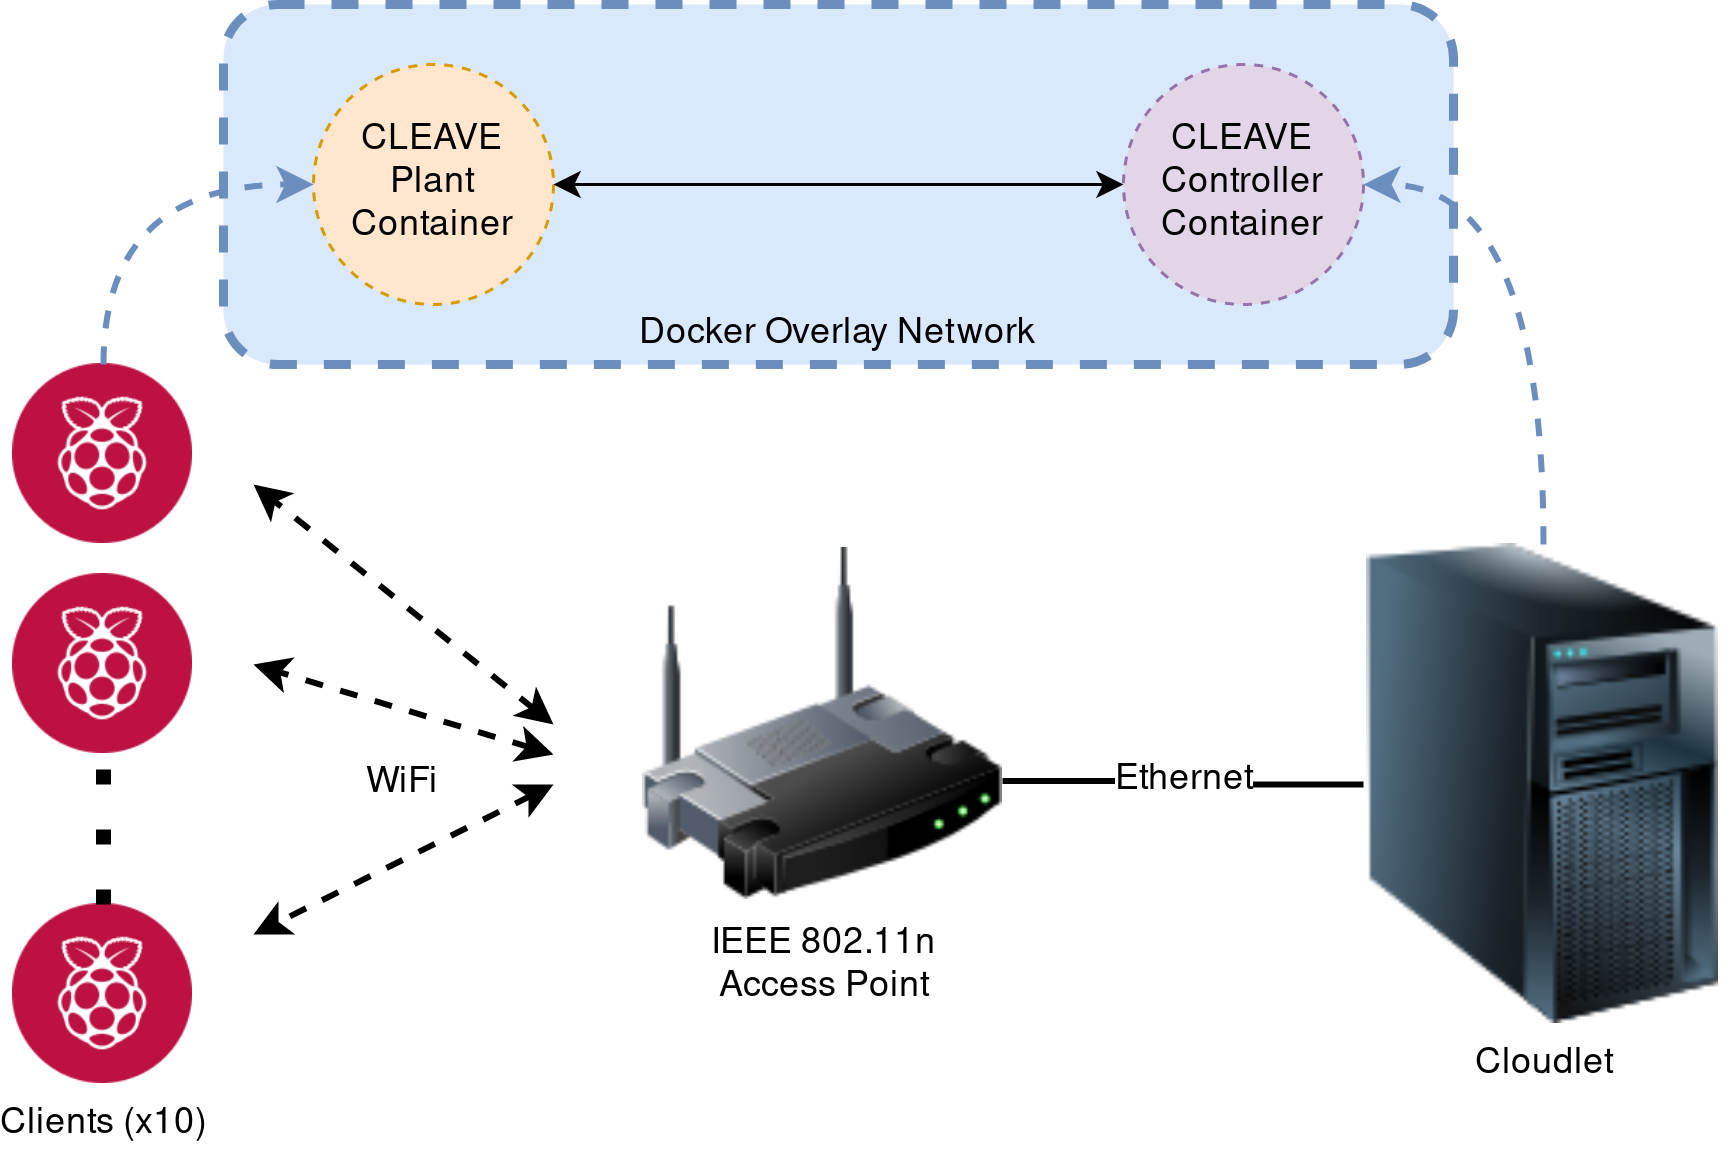
\includegraphics[width=.95\columnwidth]{images/CLEAVE_experiment_setup}
    \caption{
        The setup used for our experimentation. 
        % Containerized versions of the core CLEAVE emulation components are deployed inside a Docker Swarm Overlay Network spanning \num{10} Raspberry Pi 4B clients connected to a single Cloudlet over an IEEE 802.11n \ac{AP}.
    }\label{fig:cleave:expsetup}
\end{figure}

The first step in our case study is to evaluate the baseline performance of the control system, both locally and over the network.
We configure \ac{CLEAVE} to run a single loop with both plant and controller co-located on the Edge server, and we also configure a separate setup with an identical loop executed over the wireless link.
For both of these setups, we execute a series of scenarios varying:
\begin{enumerate*}[itemjoin={{; }}, itemjoin*={{; and }}]
    \item the sampling rate of the Plant state, setting it to \SIlist[list-final-separator={, or }]{5;10;20;40;60}{\hertz}
    \item the responsiveness of the Controller, adding fixed delays of \SIlist[list-final-separator={, or }]{0;25;50}{\milli\second} after the processing of each sample.
\end{enumerate*}

We run repeated executions of each combination of these parameters at least \num{10} times, for both the networked and ``local-only'' setups.
Each execution lasts for \SI{5}{\minute}, during which we collect detailed data on both the state of the controlled system as well as on the data sent over the network.
After the initial \num{10} runs, we identify that setups with sampling rates of \SIlist{5;10}{\hertz} were consistently too unstable to consider, and disregard them in further analyses.
We further note that setups with \SI{0}{\milli\second} additional delay are always stable and thus also disregard them.
Remaining setups, i.e.\ sampling rates \( \geq \) \SI{20}{\hertz} and artificial delays \( \geq \) \SI{25}{\milli\second}, are repeated an additional \num{20} times for better statistical significance.

This repeated experimentation and data collection while ``zooming in'' on particular setups is facilitated by \ac{CLEAVE}'s design.
Scenarios are executed automatically in batches using a simple Python script which interacts with Docker through the widely adopted \emph{docker-py}\footnote{Docker SDK for Python: \url{https://docker-py.readthedocs.io/en/stable/}} library.
This is \ac{CLEAVE}'s first advantage over existing frameworks; it is designed with cloud and edge technology and paradigms in mind, making integration with existing systems convenient.

\begin{figure}[t]
    \centering
    \begin{subfigure}[t]{\columnwidth}
        \centering
        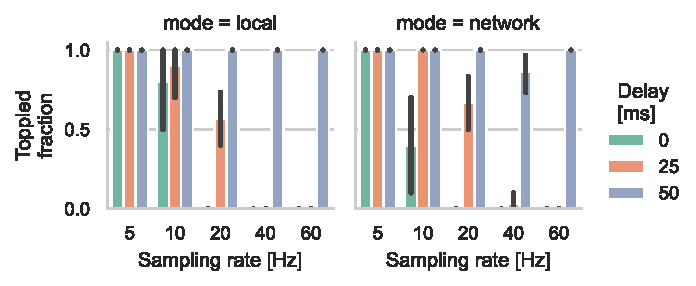
\includegraphics[width=\textwidth]{fixed_single_loop_toppled}
        \caption{Fraction of toppled plants.}\label{fig:single:topple}
    \end{subfigure}\\
    \begin{subfigure}[t]{\columnwidth}
        \centering
        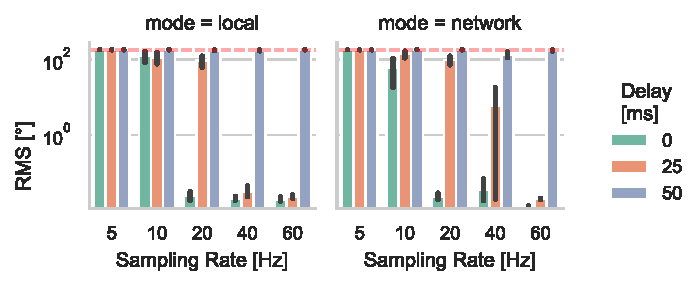
\includegraphics[width=\textwidth]{fixed_single_loop_rms}
        \caption{Mean angle \acs*{RMS}; red line indicates \( y = 180 \).}\label{fig:single:rms}
    \end{subfigure}\\
    \begin{subfigure}[t]{\columnwidth}
        \centering
        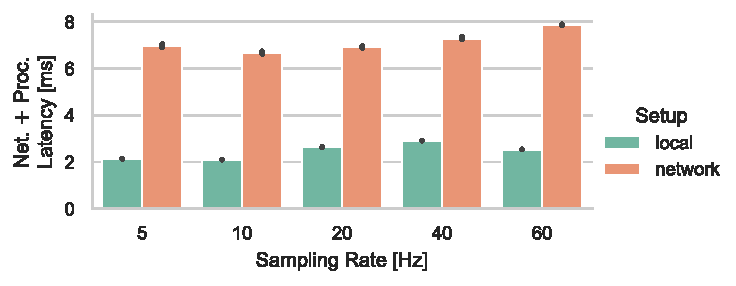
\includegraphics[width=\textwidth]{fixed_single_loop_rtts}
        \caption{
            Mean \acsp*{RTT}.
        }\label{fig:single:rtt}
    \end{subfigure}%
    \caption[caption]{
        Baseline results.
        Error bars indicate \SI{95}{\percent} \acp{CI}.
        }%
    \label{fig:single}
\end{figure}

\cref{fig:single} shows a summary of the results relating to the single-loop scenarios:
\cref{fig:single:topple} shows the fraction of plants that toppled in each scenario, and \cref{fig:single:rms} shows the average \ac{RMS} for the absolute pendula angles.
\cref{fig:single:rtt} shows average latency due to network and processing (excluding synthetic delays) for both single-loop scenarios.
Packet losses were below \SI{0.2}{\percent} for all parametrizations of the single-loop scenario over the network, and \SI{0}{\percent} for all parametrizations of the local-only setup.

As expected, higher sampling rates tend to correlate with better quality of control; at higher sampling rates the system was able to reach stability at higher \acp{RTT}.
These initial results already hint at interesting consequences for such an edge-bound \ac{NCS} deployment.
For instance, it is clear from \cref{fig:single:topple,fig:single:rms} that network delays can, to a certain extent, be compensated for by increasing the sampling rate of the system.
A corollary of this is, conversely, that at lower network latencies \acp{NCS} are able to stabilize at lower sampling rates.
Adaptive sampling might thus be a viable method for optimizing resource utilization.

Once baselines for single loops in the use case scenario have been established, we can proceed to studying the interaction between the \acp{NCS} and the video-streaming applications.
We deploy \num{6} control loops on the experimental setup depicted in \cref{fig:cleave:expsetup}.
On the remaining \num{4} clients we run the \emph{iperf3}\footnote{iperf3: \url{https://iperf.fr/}} traffic load generator, each generating \SI[per-mode=symbol]{6.5}{\mega\bit\per\second} of uplink \ac{UDP} traffic.
This emulates the load generated on the network by \SI{1080}{p} Full-HD video streaming, originating from the clients and terminating in the cloudlet.
Based on the baseline results, we execute setups with \ac{NCS} plant sampling rates of \SIlist{20;40;60}{\hertz}.
Each sampling rate configuration is run for \SI{5}{\minute}, and then repeated \num{30} times to obtain statistical significance.
Once again, repetitions of this scenario are executed automatically in batches using a simple Python script and \emph{docker-py}.

\begin{figure}[t]
    \centering
    \begin{subfigure}[h]{.22\textwidth}
        \centering
        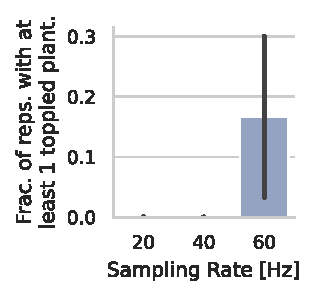
\includegraphics[width=\textwidth]{fixed_video_topple_frac}
        \caption{Toppled plants.}\label{fig:video:toppled}
    \end{subfigure}%
    \hfill%
    \begin{subfigure}[h]{.22\textwidth}
        \centering
        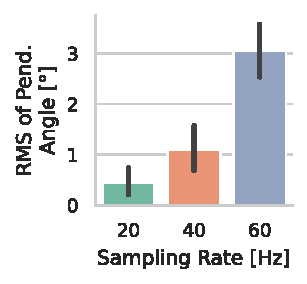
\includegraphics[width=\textwidth]{fixed_video_angle_rms}
        \caption{Angle \ac{RMS}.}\label{fig:video:rms}
    \end{subfigure}\\
    \begin{subfigure}[h]{.22\textwidth}
        \centering
        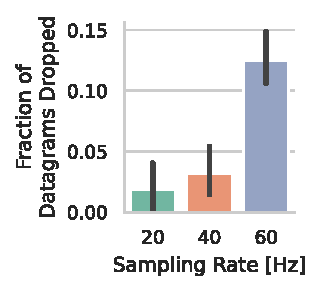
\includegraphics[width=\textwidth]{fixed_video_drop_frac}
        \caption{Packet losses.}\label{fig:video:drop}
    \end{subfigure}%
    \hfill%
    \begin{subfigure}[h]{.22\textwidth}
        \centering
        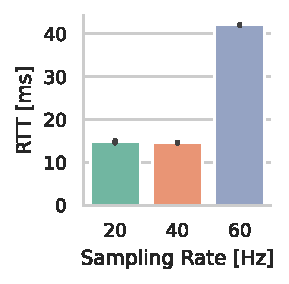
\includegraphics[width=\textwidth]{fixed_video_rtt}
        \caption{\acsp{RTT}.}\label{fig:video:rtt}
    \end{subfigure}%
    \caption{
        Multi-loop, resource-constrained setup results.
        Error bars indicate \SI{95}{\percent} \acp{CI} in all plots.
    }\label{fig:video:results}
\end{figure}

\cref{fig:video:results} shows a summary of the results obtained.
\cref{fig:video:toppled} shows the fraction of repetitions of each setup in which \emph{at least} one plant failed to maintain stability and toppled.
\cref{fig:video:rms} shows the \ac{RMS} for the pendulum angles for each setup, only considering data from plants that did not topple.
\cref{fig:video:drop} shows the fraction of \ac{UDP} datagrams dropped, averaged over all plants and repetitions per setup.
\cref{fig:video:rtt} shows the measured end-to-end plant-side \ac{RTT}, averaged over all plants and repetitions per setup.

These results are interesting in their counter-intuitiveness compared to the single-loop baseline results.
While the baselines might lead us to think that higher sampling rates are always better for the stability of control systems, \cref{fig:video:toppled,fig:video:rms} show this not to be the case for \ac{NCS} in resource-constrained scenarios.
\SI{60}{\hertz} was the least stable configuration, with at least one pendulum toppling in around \SI{16}{\percent} of the repetitions, and mean pendulum angle \ac{RMS} circa \num{3} times that of the \SI{40}{\hertz} scenario.
\SI{40}{\hertz} was in turn the second worst configuration --- although it presented no toppled pendula, average angle \ac{RMS} doubled that of the \SI{20}{\hertz} setup.

\cref{fig:video:drop,fig:video:rtt} explains these behaviors.
Whereas both the \SIlist{20;40}{\hertz} setups show losses well below \SI{5}{\percent}, the \SI{60}{\hertz} scenario shows an average of around \SI{13}{\percent} of datagrams lost.
The differences in \acp{RTT} results are equally telling; \acp{RTT} for the \SI{60}{\hertz} setup were on average approx.\ \num{3} times those for the \SIlist{20;40}{\hertz} setups.
These results stem from the contention for network resources, and hint at important trade-offs system designers will have to take into consideration when designing and developing \acp{NCS} for deployment on the Edge.
The Edge will be \emph{multi-tenant} and \emph{multi-instance}. 
\ac{NCS} deployments will have to be designed with shared resources in mind, and given the complexity of these systems, experimental tools like \ac{CLEAVE} will be key for their succesful adoption and massification.
